\newcommand{\tbontype}{\textsc{tbon}\textunderscore \textsc{tc}\textunderscore  \textsc{type}}
\newcommand{\tbonclasstype}{\textsc{tbon}\textunderscore \textsc{tc}\textunderscore \textsc{class}\textunderscore  \textsc{type}}
\newcommand{\tbonclustertype}{\textsc{tbon}\textunderscore \textsc{tc}\textunderscore \textsc{cluster}\textunderscore  \textsc{type}}
\newcommand{\tbonfeature}{\textsc{tbon}\textunderscore \textsc{tc}\textunderscore \textsc{feature}}
\newcommand{\tbongeneric}{\textsc{tbon}\textunderscore \textsc{tc}\textunderscore \textsc{generic}}

\section{Type Checker}
Test
\label{implementation-def-boolean-type}
\label{implementation-set-expressions}


\subsection{Building the Context}
\label{implementation-context-class-structure}
The type contexts for type checking of both informal and formal specifications are built using a hierarchy of types. This hierarchy is shown in figure \ref{fig:context-classes}.
\begin{figure}[H]
    \scalebox{0.6}{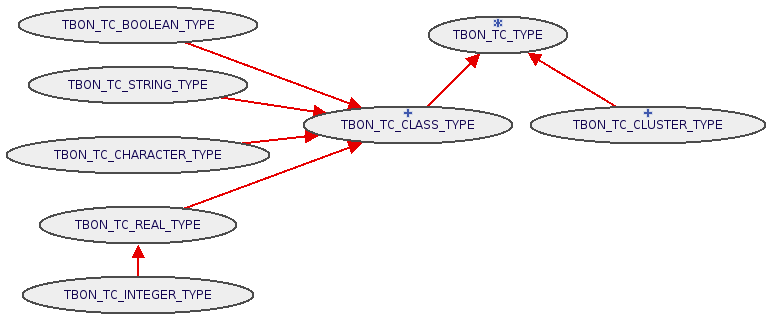
\includegraphics{images/context_classes3.png}}
    \caption[Context classes]{Hierarchy of classes used to build the type contexts}
    \label{fig:context-classes}
\end{figure}
A context, be it informal or formal, is built as a set of instances of \tbonclasstype   and \tbonclustertype   (declared as a set of \tbontype ). Due to the naming restrictions discussed in section \ref{design-type-names}, classes and clusters are kept in the same context for convenience and easy detection of name clashes. At any time, the instances in the context represent the defined types currently known at that point.
\paragraph{} Mapping from classes to features (in formal specifications) happens through association with a set of \tbonfeature . An instance of \tbonclasstype  is never associated with an undefined feature, but can be associated with an inconsistent or ill-typed feature (elaboration on this is found in section \ref{implementation-unresolved-elements}). Accordingly, the type of a feature is merely an association to an instance of \tbonclasstype .
\paragraph{} Analogous to the mapping from classes to features, mapping from classes to generics is done through association with a sequence of \tbongeneric  (generics cannot be stored in a set, as the order of the type parameters matters). A generic type has both a bounding and an actual class type. The association between these is explained in section \ref{implementation-generics}.

\subsection{Going Through the Phases}
\subsubsection{Unresolved Elements}
\label{implementation-unresolved-elements}

%Generics - explain association between bounding type and actual type.
\label{implementation-generics}
\subsection{Inheritance}

An important part of type checking textual \textsc{bon} is checking the inheritance. Apart from the obvious things such as checking whether an ancestor class actually exists, it is also important to check for circular inheritance. A class cannot inherit from itself, even through other classes. This means that the type checker has to check not only the direct ancestors of the class in question, but also all their direct ancestors and so. This is implemented with a recursive algorithm. Before implementing it the algorithm was written in pseudocode, as seen in figure \ref{fig:check_ancestors_pseudocode}.
\begin{figure}[h]
{\footnotesize
\begin{verbatim}
 1| check_ancestors(main_class, current_class): BOOLEAN
 2|      do
 3|           Result := current_class.ancestors.for_all(ancestor /= main_class)
 4|           if Result then
 5|                Result := current_class.ancestors.for_all(
 6|                                            check_ancestors(main_class, ancestor)
 7|                                            )
 8|           else
 9|                Result := False
10|                error_msg("circular inheritance")
11|           end
12|      end
\end{verbatim}
}
\caption{Pseudo-code for check\textunderscore ancestors}
\label{fig:check_ancestors_pseudocode}
\end{figure}

In the first iteration \textit{main}\textunderscore\textit{class} and \textit{current}\textunderscore\textit{class} are both the root class. First the direct ancestors of the \textit{current}\textunderscore\textit{class}  is checked for presences of the \textit{main}\textunderscore\textit{class}. If this does not pass an error message is created and the algorithm terminates. If it does pass the algorithm will continue to check all ancestors of \textit{current}\textunderscore\textit{class}. This is done by recursively calling the feature with each ancestor as \textit{current}\textunderscore\textit{class}. It is important to note that \textit{main}\textunderscore\textit{class} does not change through out the recursive iterations. It is always checking in relation to the same class.

\begin{figure}
\centerline{
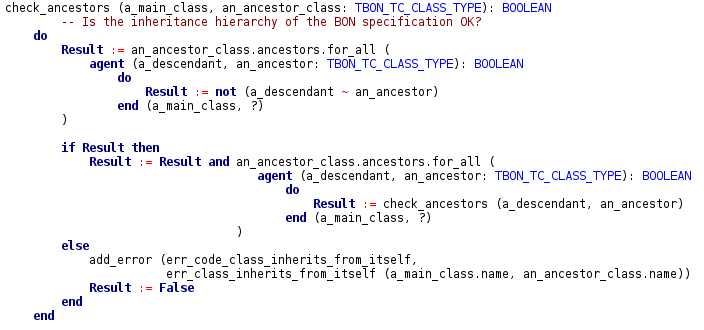
\includegraphics[scale=0.7]{images/check_ancestors_eiffel_code.png}
}
\caption{Eiffel implementation of the \textit{check}\textunderscore\textit{ancestors} algorithm}
\label{fig:eiffel_check_ancestors}
\end{figure}

\paragraph{}
In figure \ref{fig:eiffel_check_ancestors} the actual implementation in Eiffel is shown. The most notable difference between the implementation and the pseudocode is that when the it is iterating through the ancestors to call \textit{check}\textunderscore\textit{ancestors} on the ancestors, it is \textbf{and}'ed with \textbf{Result}. This does not change how the program works, due to the conditional statement ensuring that \textbf{Result} always is \textbf{True} at that point. It is done to express that the value of \textbf{Result} does not only depend on the returned value of the expression, but also on the previous evaluation of the direct ancestors. This means that the conditional statement could have been excluded, but as it stops the algorithm from further unnecessary iterations when a type error has been found, it is included.

Lastly, the error handling is done by the type checkers error handling section. This will be further described in section \ref{error_section}.
\import{./}{implementation-informal-bon}

\subsection{Error handling}
\label{error_section}